%%
%% Author: dariochinelli
%% 2020-10-13
%%

\section{Principio di Esclusione di Pauli}

Si consideri una scatola contenente due particelle. In Fisica Classica è sempre possibile distinguere il moto dell'una da quella dell'altra.
In Meccanica Quantistica invece, a causa del Principio di Indeterminazione, le due particelle sono indistinguibili poiché le due funzioni d'onda si sovrappongono.
Dunque occorre richiedere che tutti i risultati quanto-meccanici non devono perciò dipendere dall'assegnare un'etichetta a una particella piuttosto che ad un'altra.
È necessario scrivere quindi funzioni d'onda che tengano conto della instabilità delle particelle, le quali non interagiscono fra loro.
Partiamo scrivendo l'equazione di Schrodinger indipendente dal tempo per le due particelle:

\begin{equation}
- \frac{\hbar^2}{2m} \Bigl(  \frac{\partial^2 \Psi_T}{\partial x_1^2} + \frac{\partial^2 \Psi_T}{\partial y_1^2} + \frac{\partial^2 \Psi_T}{\partial z_1^2}  \Bigr) 
- \frac{\hbar^2}{2m} \Bigl(  \frac{\partial^2 \Psi_T}{\partial x_2^2} + \frac{\partial^2 \Psi_T}{\partial y_2^2} + \frac{\partial^2 \Psi_T}{\partial z_2^2}  \Bigr) 
+ V_T \Psi_T = E_T \Psi_T
\end{equation}

$$\mbox{In cui il potenziale usato è: } V_T = V(x_1, y_1, z_1) + V(x_2, y_2, z_2) $$

$$\mbox{In cui la funzione d'onda usata è: } \Psi_T = \Psi(x_1, y_1, z_1) \Psi(x_2, y_2, z_2) = \Psi_\alpha(1) \Psi_\beta(2)$$

Servono 3 numeri quantici per indicare le coordinate spaziali.
Poiché le particelle non sono distinguibili si potrebbe avere la particella 2 nello stato $\alpha$ e, viceversa, la particella 1 nello stato $\beta$.

Per la funzione d'onda è:

$$ \mbox{ 1) } \Psi_T = \Psi_\alpha(1) \Psi_\beta(2) $$
$$ \mbox{ 2) } \Psi_T = \Psi_\beta(1) \Psi_\alpha(2) $$

Cerchiamo la densità di probabilità della 1) e della 2):

$$ \mbox{ 3) } \Psi_\alpha^\ast(1) \Psi_\beta^\ast(2) \Psi_\alpha(1) \Psi_\beta(2) $$
$$ \mbox{ 4) } \Psi_\beta^\ast(1) \Psi_\alpha^\ast(2) \Psi_\beta(1) \Psi_\alpha(2) $$

Se scambio le "etichette" nella 3) cosa ottengo?

$$ \Psi_\alpha^\ast(2) \Psi_\beta^\ast(1) \Psi_\alpha(2)  \Psi_\beta(1) $$

che è un risultato diverso! Ciò significa che non tiene conto della indisitinguibilità.
Esistono due modi per scrivere funzioni d'onda che tengono conto di questo fatto:

$$ \mbox{a) } \Psi_s = \frac{1}{\sqrt{2}} \Bigl[ \Psi_\alpha(1) \Psi_\beta(2) + \Psi_\beta(1) \Psi_\alpha(2) \Bigr] \mbox{ soluzione simmetrica} $$
$$ \mbox{b) } \Psi_a = \frac{1}{\sqrt{2}} \Bigl[ \Psi_\alpha(1) \Psi_\beta(2) - \Psi_\beta(1) \Psi_\alpha(2) \Bigr] \mbox{ soluzione antisimmetrica} $$

Si tratta di due autofunzioni diverse per la stessa energia totale: si chiama \underline{degenerazione di scambio}
(dove per "scambio" si intende lo scambio delle "etichette").

Scambiamo quindi le etichette: 
$ 1 \to 2 $ e $ 2 \to 1 $

$$ \mbox{a) } \frac{1}{\sqrt{2}} \Bigl[ \Psi_\alpha(2) \Psi_\beta(1) + \Psi_\beta(2) \Psi_\alpha(1) \Bigr] = \Psi_s $$
$$ \mbox{b) } \frac{1}{\sqrt{2}} \Bigl[ \Psi_\alpha(2) \Psi_\beta(1) - \Psi_\beta(2) \Psi_\alpha(1) \Bigr] = - \Psi_a $$

Si dimostra che la densità di probabilità non cambia:

\begin{equation}
\begin{cases}
	\Psi_s^+ \Psi_s \to \Psi_s^\ast \Psi_s \\
	\Psi_a^+ \Psi_a \to (-1)^2 \Psi_a^\ast \Psi_a = \Psi_a^\ast \Psi_a
\end{cases}
\end{equation}

Nel 1925, Pauli preannuncia il suo celebre Principio di Esclusione: non ci può essere, nei sistemi multi elettronici, più di un elettrone in uno stesso stato quantico.

Cercando il contrario:
$$ \Psi_a = \frac{1}{\sqrt{2}} \Bigl[ \Psi_\alpha(1) \Psi_\alpha(2) - \Psi_\alpha(1) \Psi_\alpha(2) \Bigr] = 0 $$

Dunque la probabilità di trovare due elettroni nello stesso stato è nulla.
Se ne deduce che le particelle descritte da funzioni d'onda antisimmetriche, sono soggette al Principio di Esclusione di Pauli.
Tuttavia non tutte le particelle si comportano così, sperimentalmente si ricava la seguente tabella:

\begin{figure}[h]
\centering
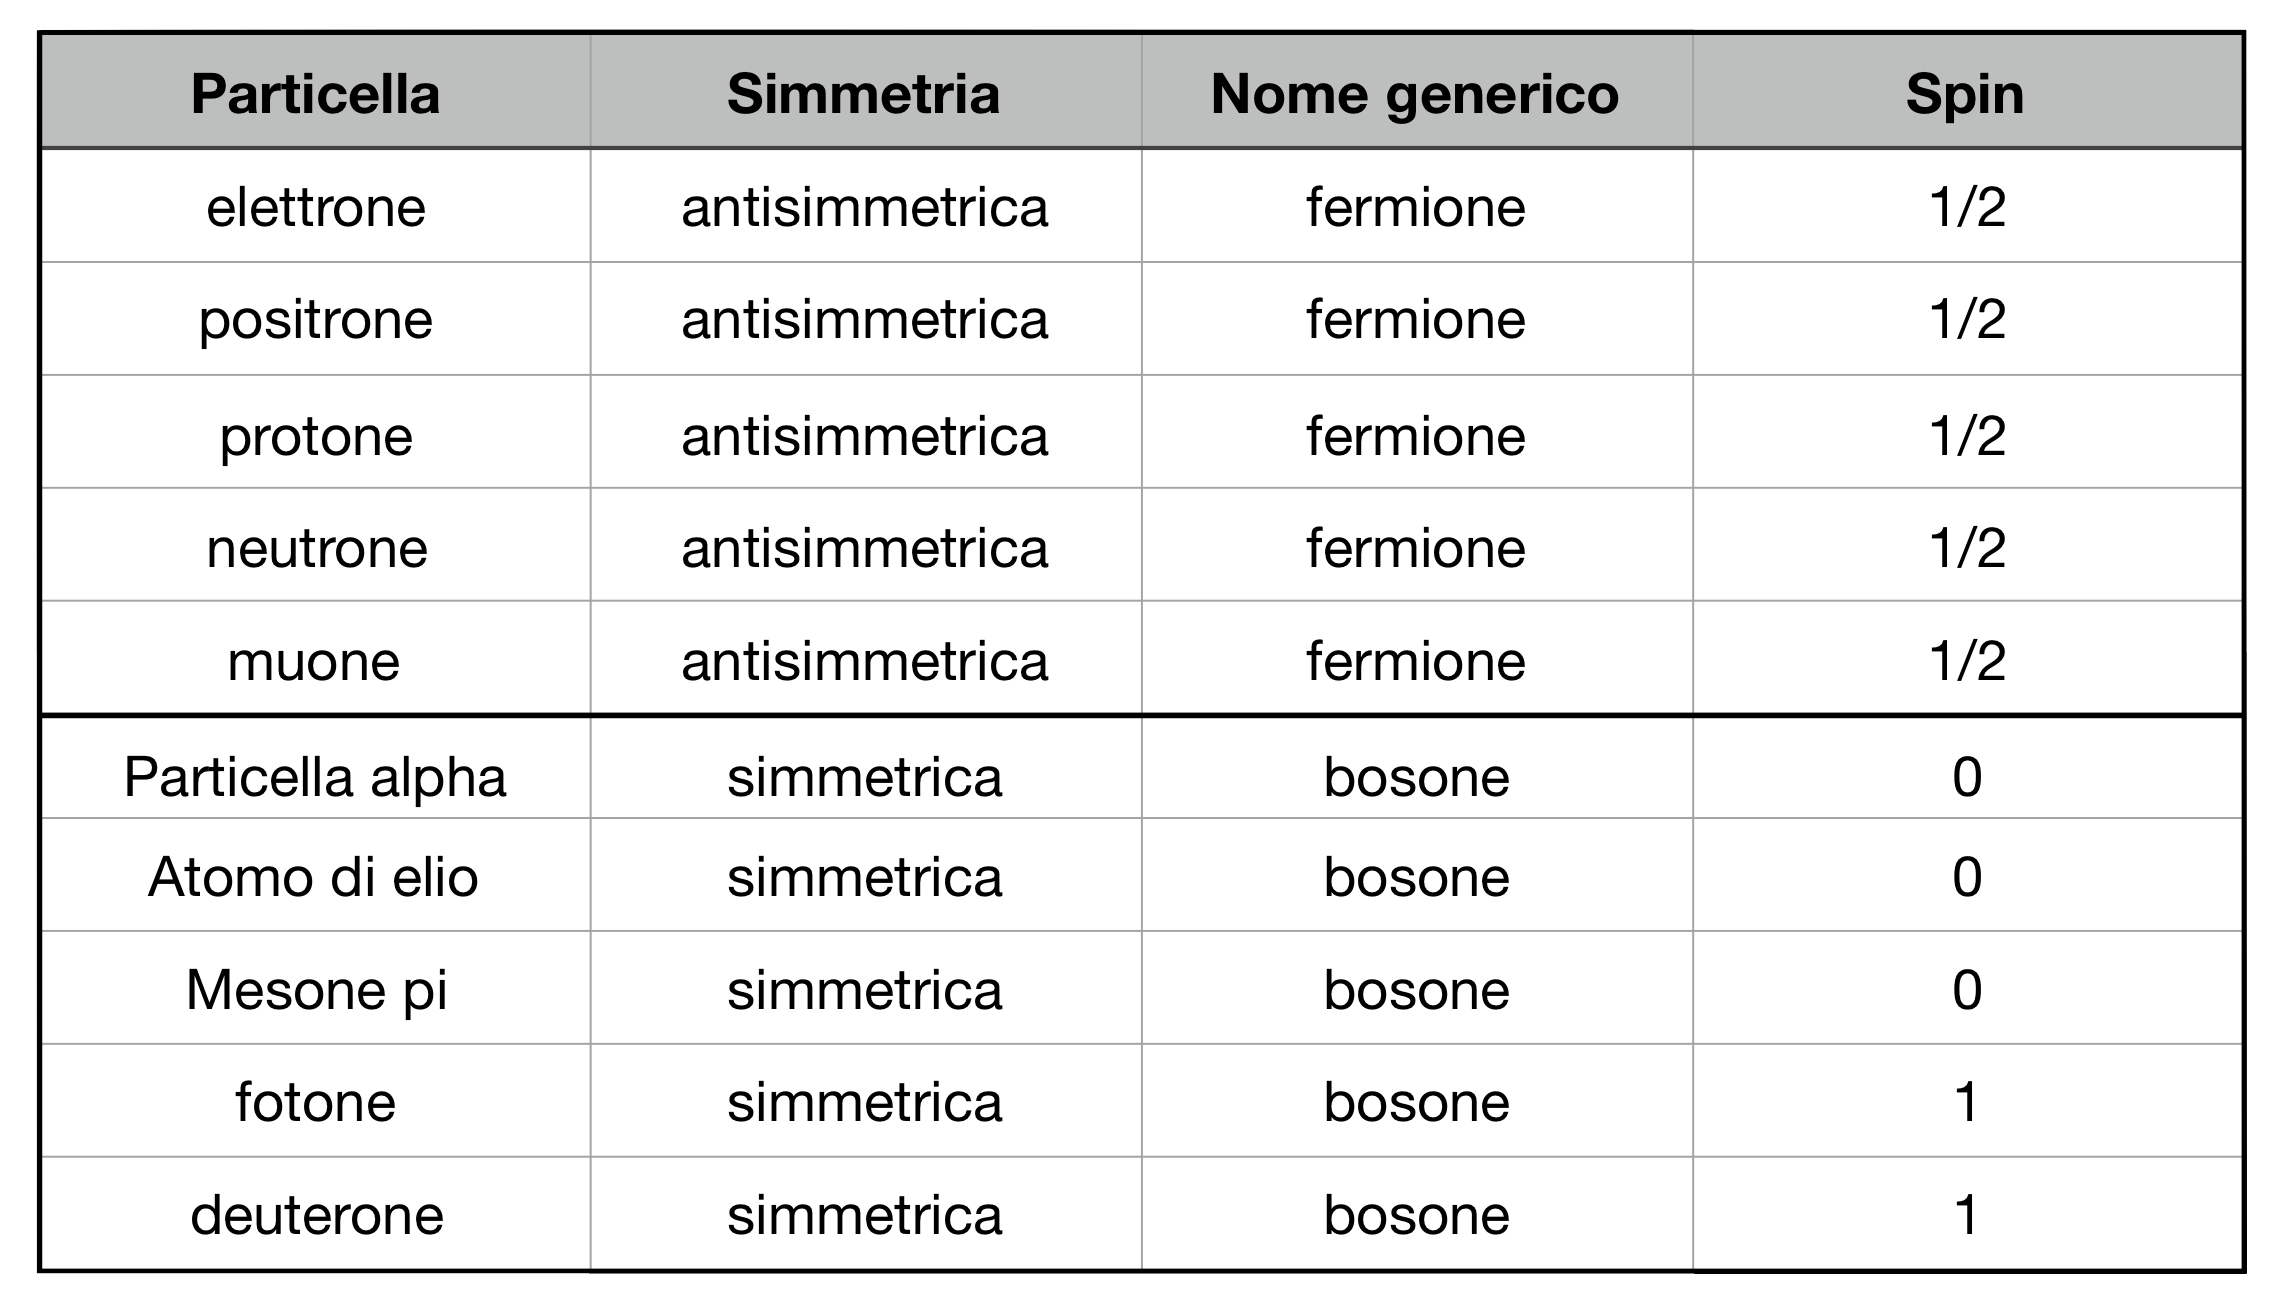
\includegraphics[scale=0.7]{/particelle_simm_spin}
\caption{Tabella delle funzioni d'onda di alcune particelle note e spin}
\end{figure}

I \underline{bosoni} sono dunque particelle descritte da funzioni d'onda simmetriche ed i \underline{fermioni} da funzioni d'onda antisimmetriche.
Se si suppone che due particelle siano nello stesso stato quantico $(\alpha = \beta)$, allora si ha che:

$$ \Psi_T^\ast \Psi_T = \Psi_\beta^\ast(1) \Psi_\beta^\ast(2) \Psi_\beta(1) \Psi_\beta(2) $$

Nel caso di funzioni d'onda simmetriche si ottiene che la densità di probabilità è:

$$ \Psi_s^\ast \Psi_s = 2 \Psi_\beta^\ast(1) \Psi_\beta^\ast(2) \Psi_\beta(1) \Psi_\beta(2) = 2 \Psi_T^\ast \Psi_T \not = 0 $$

Se considero quindi due bosoni indistinguibili, la probabilità di trovarli in un certo stato è il doppio rispetto alla probabilità calcolata senza tenere conto della non distinguibilità.










